\chapter{Conservation of Linear Momentum}

Date: 29/10/2020

\section{Aim}

In this experiment we aim to observe the final velocities of two trolleys, on a track using light gates, that are colliding elastically and in-elastically by varying their masses. We observe their initial velocity and make inferences using data from CASSY software. 


\section{Background Theory}

We define Linear momentum for a object of mass m kg and velocity $\vec{v}$ to be 
$$ \vec{p} = m \times \vec{v} $$
The principle of conservation of momentum states that ``If no net force acts upon a system, then there is no change in the total momentum of the system.''. This can be expressed mathematically as 
$$ \vec{p_{initial}} = \vec{p_{final}}$$
In case of an elastic collision, the total momentum and the kinetic energy before and after the collision is conserved. This can be expressed as 
$$ m_1 \times \vec{v_{i^1}} +  m_2 \times \vec{v_{i^2}} =  m_1 \times \vec{v_{f^1}} +  m_2 \times \vec{v_{i^2}}$$
$$ \frac{1}{2} \times( m_1 \times (\vec{v_{i^1}})^2 +  m_2 \times (\vec{v_{i^2}})^2 ) =  \frac{1}{2} \times( m_1 \times (\vec{v_{f^1}})^2 +  m_2 \times (\vec{v_{i^2}})^2) $$
In case of an in-elastic collision, only the total momentum is conserved. This can be expressed as 
$$ m_1 \times \vec{v_{i^1}} +  m_2 \times \vec{v_{i^2}} =  (m_1 + m_2 ) \times\vec{v_f}$$

Elastic Collision and $m1 = m2$ . 
\begin{center}
    \begin{itemize}
        \item $ \vec{v_{f^1}} = \vec{v_{i^2}}$
        \item $ \vec{v_{f^2}} = \vec{v_{i^i}}$
    \end{itemize}
\end{center}

Elastic Collision and $m1 \neq m2$ . 
\begin{center}
    \begin{itemize}
        \item $ \vec{v_{f^1}} = \frac{m_1 - m_2}{m_1+m_2} \times \vec{v_{i^i}} +  \frac{2 \times m_2 \vec{v_{i^2}}}{m1+m2}$
        \item $ \vec{v_{f^2}} = \frac{m_2 - m_1}{m_1+m_2} \times \vec{v_{i^1}} +  \frac{2 \times m_1 \vec{v_{i^1}}}{m1+m2}$
    \end{itemize}
\end{center}
In-Elastic Collision and $m1 = m2$ . 
\begin{center}
    \begin{itemize}
        \item $ \vec{v_{f}} = 0.5 \times \vec{v_{i^2}}$
    \end{itemize}
\end{center}
In-Elastic Collision and $m1 \neq m2$ . 
\begin{center}
    \begin{itemize}
        \item $ \vec{v_{f}} = \frac{(m_1 \times \vec{v_{i^1}} +  m_2 \times \vec{v_{i^2}})}{m_1 + m_2}$
    \end{itemize}
\end{center}

\section{Description of Setup}
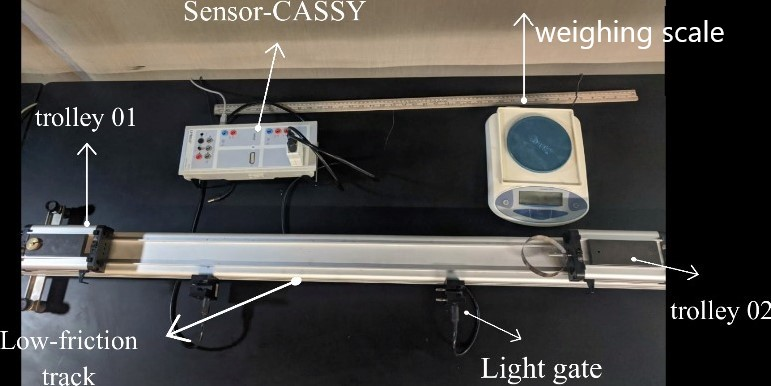
\includegraphics[width=15cm, height=8cm]{figures/exp5fig.jpeg} \\
In the setup above two trolleys with additional weights are placed on a track with light gates. Cassy Software is attached to record data and an electronic balance is used to measure the mass of trolleys.  

% Sketch and explain the experimental setup. The explanation should try to cover these pointers:  table \ref{tab:addlabel}
% \begin{enumerate}
%     \item What is the purpose of individual items in the setup?
%     \item If any equipment is taking measurements, what is it reading and how is it being read?
% \end{enumerate}

% Be precise to, ONLY include scientific description.

\section{Method / Procedure}
The CASSY software settings were set up for the conservation of momentum. The masses of trolleys were measured using the balance alongside the spring for elastic collision and the two trolleys were pushed to collide elastically with equal masses. This was repeated five times. Elastic collision was also performed using unbalanced masses and velocities data was seen through CASSY. The same procedure was repeated for inelastic collision with equal masses and unequal masses five times respectively. CASSY was used to collect the data of masses of trolleys and initial and final velocities of trolleys before and after collisions with the help of light gates. 

% Highlight the following aspects of the experiment conducted 
% \begin{enumerate}
%     \item What method did you use to perform the experiment?
%     \item What adjustments were made, if any? 
%     \item What data was collected?
%     \item How was it collected?
%     \item Were any calibrations made and what were they?
% \end{enumerate}



\section{Data}

\begin{center}
    
\begin{adjustbox}{width=1\textwidth}
\begin{tabular}{|l|l|l|l|l|l|l|}
\hline

\multicolumn{7}{|c|}{\textbf{Elastic Collision (Case a: m1 = m2)}} \\ \hline
Serial No & V1-initial - m/s & V2-initial - m/s & V1-final (experiment) - m/s & V1-final (theoretical) - m/s & V2-final (experiment) - m/s & V2-final (theoretical) - m/s \\ \hline
1   & 0.687   & -0.511   & -0.453   & -0.511   & 0.679   & 0.687   \\ \hline
2   & 0.762   & -0.83    & -0.762   & -0.83    & 0.704   & 0.762   \\ \hline
3   & 0.55    & -0.572   & -0.523   & -0.572   & 0.553   & 0.55    \\ \hline
4   & 0.637   & -0.702   & -0.634   & -0.702   & 0.63    & 0.637   \\ \hline
5   & 0.547   & -0.611   & -0.558   & -0.611   & 0.543   & 0.547   \\ \hline
\end{tabular}
\end{adjustbox}
\end{center}

\begin{center}
\begin{adjustbox}{width=1\textwidth}
\begin{tabular}{|l|l|l|l|l|l|l|}
\hline
\multicolumn{7}{|c|}{\textbf{Elastic Collision (Case b: m1 != m2)}} \\ \hline
Serial No & V1-initial - m/s & V2-initial - m/s & V1-final (experiment) - m/s & V1-final (theoretical) - m/s & V2-final (experiment) - m/s & V2-final (theoretical) - m/s \\ \hline
1  & 0.573  & -0.616  & -0.178 & -0.210155718 & 0.936 & 0.978844282 \\ \hline
2  & 0.594  & -0.538  & -0.154 & -0.151611667 & 0.848 & 0.980388333 \\ \hline
3  & 0.411  & -0.477  & -0.156 & -0.173896785 & 0.691 & 0.714103215 \\ \hline
4  & 0.393  & -0.694  & -0.299 & -0.322971627 & 0.731 & 0.764028373 \\ \hline
5  & 0.491  & -0.566  & -0.18  & -0.205211601 & 0.827 & 0.851788399 \\ \hline
\end{tabular}
\end{adjustbox}
\end{center}

\begin{center}
\begin{adjustbox}{width=1\textwidth}
\begin{tabular}{|l|l|l|l|l|l|l|}
\hline
\multicolumn{7}{|c|}{\textbf{In-Elastic Collision (Case a: m1 = m2)}} \\ \hline
Serial No & V1-initial - m/s & V2-initial - m/s & V1-final (experiment) - m/s & V1-final (theoretical) - m/s & V2-final (experiment) - m/s & V2-final (theoretical) - m/s \\ \hline
1     & 0.535    & 0    & 0.26     & 0.2675    & 0.262    & 0.2675    \\ \hline
2     & 0.677    & 0    & 0.331    & 0.3385    & 0.332    & 0.3385    \\ \hline
3     & 0.693    & 0    & 0.337    & 0.3465    & 0.345    & 0.3465    \\ \hline
4     & 0.584    & 0    & 0.258    & 0.292     & 0.263    & 0.292     \\ \hline
5     & 0.616    & 0    & 0.298    & 0.308     & 0.301    & 0.308     \\ \hline
\end{tabular}
\end{adjustbox}
\end{center}

\begin{center}
\begin{adjustbox}{width=1\textwidth}
\begin{tabular}{|l|l|l|l|l|l|l|}
\hline
\multicolumn{7}{|c|}{\textbf{In-Elastic Collision (Case b: m1 != m2)}} \\ \hline
Serial No & V1-initial - m/s & V2-initial - m/s & V1-final (experiment) - m/s & V1-final (theoretical) - m/s & V2-final (experiment) - m/s & V2-final (theoretical) - m/s \\ \hline
1   & 0.559  & -0.521  & 0.196  & 0.199193133  & 0.196  & 0.199193133  \\ \hline
2   & 0.441  & -0.424  & 0.151  & 0.152821352  & 0.152  & 0.152821352  \\ \hline
3   & 0.512  & -0.511  & 0.172  & 0.17118294   & 0.173  & 0.17118294   \\ \hline
4   & 0.454  & -0.539  & 0.117  & 0.123177575  & 0.12   & 0.123177575  \\ \hline
5   & 0.51   & -0.328  & 0.23   & 0.230816524  & 0.232  & 0.230816524  \\ \hline
\end{tabular}
\end{adjustbox}
\end{center}



\section{Data Analysis}
\newpage
\begin{figure}[h!]
    \centering
    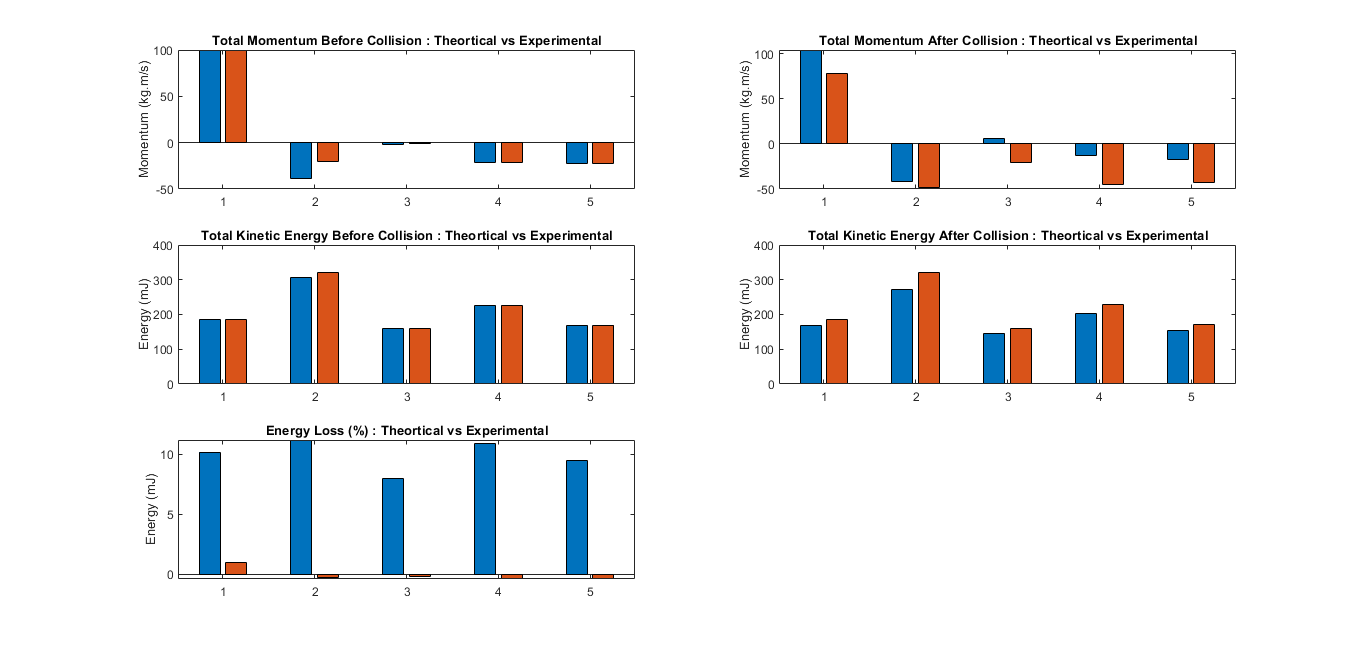
\includegraphics[width=\textwidth]{figures/Exp1.png}
    \caption{Elastic Collision with $m_1 = m_2$}
    \label{fig:yx}
\end{figure}

\newpage
\begin{figure}[h!]
    \centering
    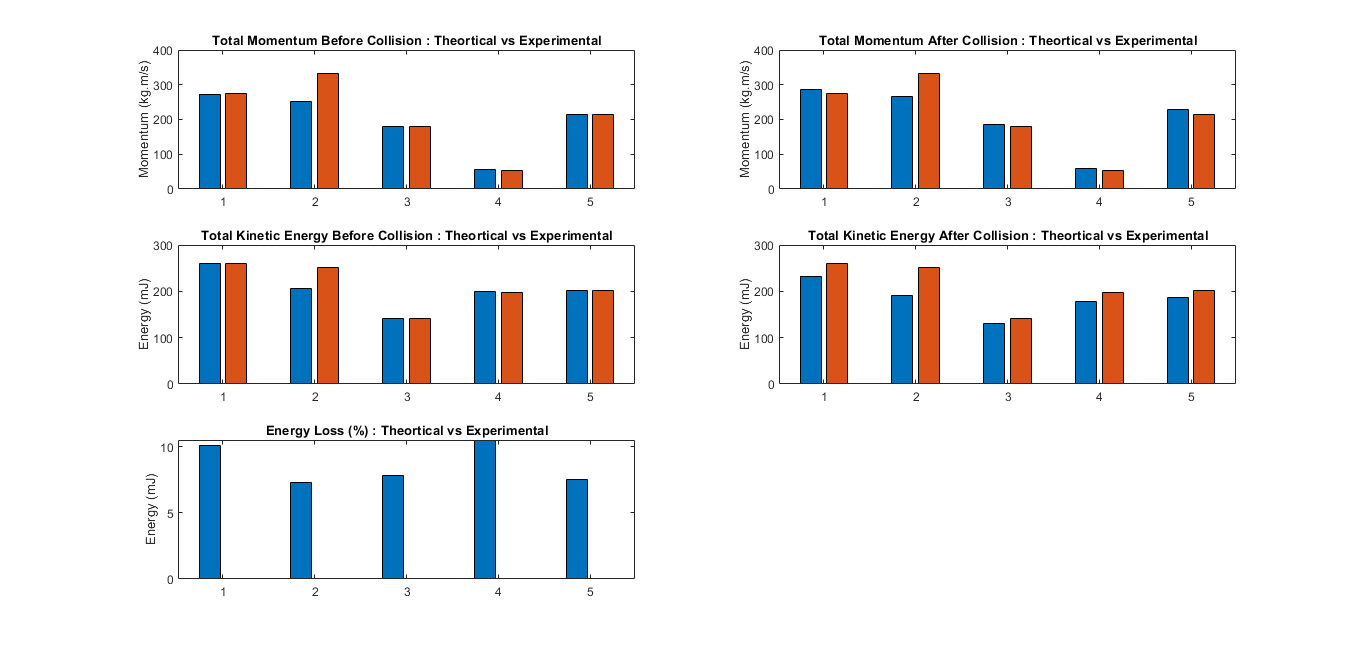
\includegraphics[width=\textwidth]{figures/Exp2.png}
    \caption{Elastic Collision with $m_1 \neq m_2$}
    \label{fig:yx}
\end{figure}

\newpage
\begin{figure}[h!]
    \centering
    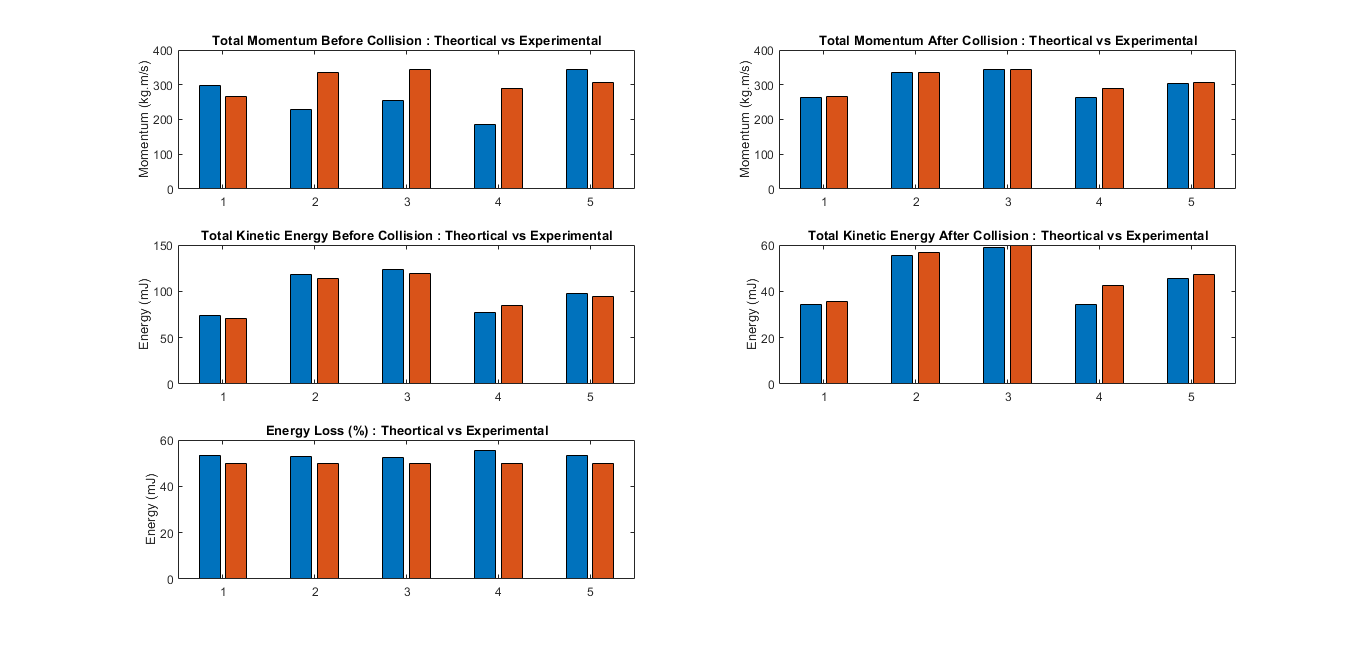
\includegraphics[width=\textwidth]{figures/Exp3.png}
    \caption{In-Elastic Collision with $m_1 = m_2$}
    \label{fig:yx}
\end{figure}
\newpage
\begin{figure}[h!]
    \centering
    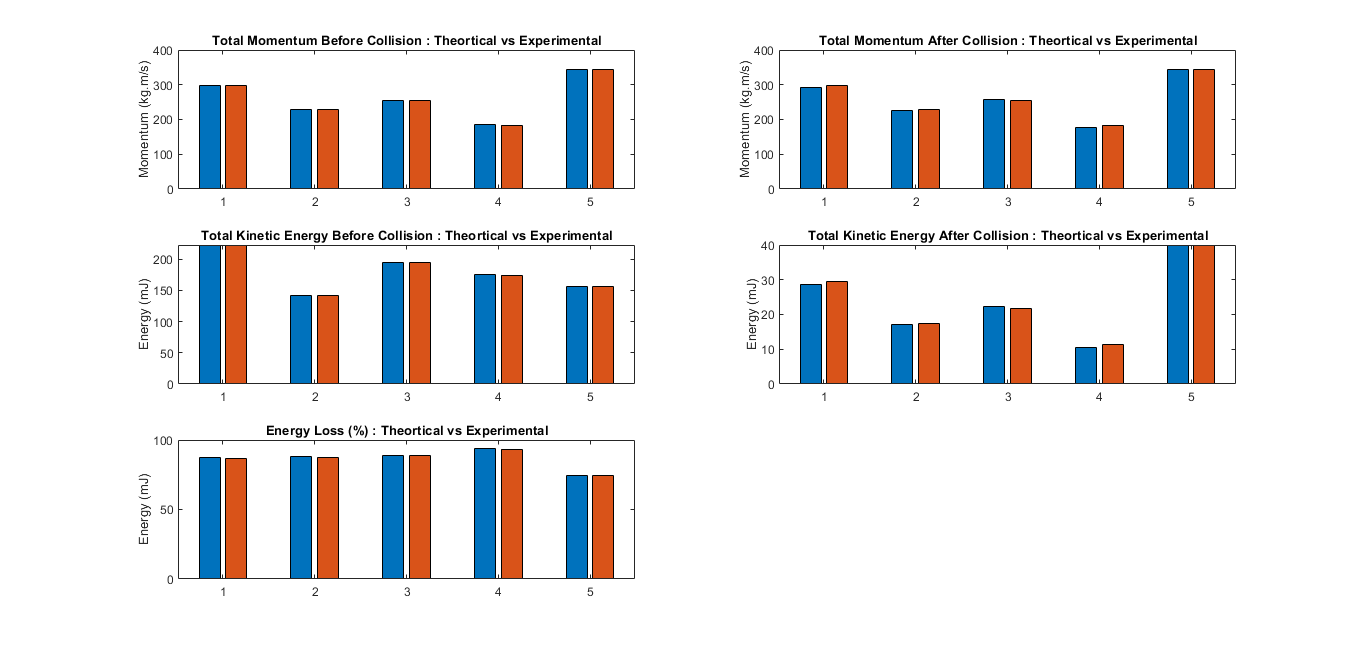
\includegraphics[width=\textwidth]{figures/Exp4.png}
    \caption{In-Elastic Collision with $m_1 \neq m_2$}
    \label{fig:yx}
\end{figure}

\section{Discussion \& Conclusion}

In both elastic and in-elastic, the experiment values agreed with the theoretical values up to a great extent when $m1\neq m2$. This is because in reality we didn't use equal masses. Moreover, elastic collisions don't occur in nature unless they are atomic in nature.



\section{MATLAB Script}
\lstinputlisting{matlabCodes/Experiment5.m}



